\section{Linear Algebra Applications}
\label{section:skelcl:evaluation:linearAlgebra}

In this section we are going to evaluate \SkelCL using two basic linear algebra applications:
\begin{itemize}
  \item the sum of absolute values of a vector and
  \item the dot product of two vectors.
\end{itemize}

Both applications are included in BLAS~\cite{Dongarra2002,Dongarra2002a}, the well known library of basic linear algebra functions.
The BLAS functions are used as basic building blocks by many HPC applications.
% Especially dense matrix multiplication is an important operation found in numerous scientific applications.

Here we want to investigate how easily these applications can be expressed with skeletons in \SkelCL.
Furthermore, we are interested in the runtime performance of the \SkelCL implementations.

\subsection*{Sum of Absolute Values}
\label{sec:asum}
\autoref{eq:asum} shows the mathematical definition of the sum of absolute values (short \emph{asum}) for a vector $\vec{x}$ of length $n$ with elements $x_i$:
\begin{equation}
  asum\ \vec{x} = \sum_{i=0}^{n} | x_i |
  \label{eq:asum}
\end{equation}
For all elements of the vector the absolute values are added up to produce the final scalar result.

\subsubsection*{\SkelCL Implementation}
In the \SkelCL programming model we can express \emph{asum} using the \map and \reduce skeletons as follows:
\begin{align}
  asum\ \vec{x} &= reduce\ (+)\ 0\ \big(\ map\ (|\, .\, |)\ \vec{x}\ \big)\label{eq:asum:skelcl}\\
  \text{where:} \qquad | a | &=
    \left\{
      \begin{array}{r l}
      a & \text{if } a \geq 0\\
      -a & \text{if } a < 0
      \end{array}
    \right.\nonumber
\end{align}
The \map skeleton applies the $(|\, .\, |)$ function to each element of the input vector before the \reduce skeleton is used to sum up the elements.

The implementation of $asum$ using the \SkelCL library is shown in \autoref{lst:skelcl:asum}.
In lines~\ref{lst:skelcl:asum:skeletons:start}--\ref{lst:skelcl:asum:skeletons:end} the customized skeletons are defined.
The \map skeleton in \autoref{eq:asum:skelcl} corresponds directly to lines~\ref{lst:skelcl:asum:skeletons:start} and~\ref{lst:skelcl:asum:abs} in \autoref{lst:skelcl:asum} where the $|\, .\, |$ function is represented using a \Cpp lambda expression.
Line~\ref{lst:skelcl:asum:skeletons:end} corresponds directly to the \reduce skeleton in \autoref{eq:asum:skelcl}.
By applying the skeletons to the input vector (line~\ref{lst:skelcl:asum:call}) the result is computed and accessed in line~\ref{lst:skelcl:asum:return}.
In the \SkelCL library implementation the \reduce skeleton returns a vector containing a single element.
The containers in the \SkelCL library are implemented as \emph{futures}~\cite{HewittBa1977,FriedmanWi1978}.
This allows the computation of all skeletons to be performed asynchronously, \ie, when executing a skeleton the computation is launched and the called function returns immediately.
When accessing values of the returned container, \eg, via the array subscript operator as shown in line~\ref{lst:skelcl:asum:return}, the call will block until the accessed value has been computed.

\begin{lstlisting}[%                                                             
caption={Implementation of the \emph{asum} application in \SkelCL},%
numbers=left,%
float=tb,
label={lst:skelcl:asum}]
float asum(const Vector<float>& x) {
  auto absAll = map($\label{lst:skelcl:asum:skeletons:start}$
      [](float a){ if (a >= 0) return a; else return -a; });$\label{lst:skelcl:asum:abs}$
  auto sumUp = reduce([](float a, float b){return a+b;}, 0);$\label{lst:skelcl:asum:skeletons:end}$
  auto result = sumUp( absAll( x ) );$\label{lst:skelcl:asum:call}$
  return result[0]; }$\label{lst:skelcl:asum:return}$
\end{lstlisting}


\subsection*{Dot Product}
\label{sec:dot}
The computation of the dot product, \aka scalar product, is a common mathematical operation performed on two input vectors $\vec{x}$ and $\vec{y}$ of identical length $n$ as defined in \autoref{eq:dot_product}:
\begin{equation}
  dotProduct\ \vec{x}\ \vec{y} = \sum_{i=0}^{n} x_i \times y_i
  \label{eq:dot_product}
\end{equation}

\subsubsection*{\SkelCL Implementation}
In the \SkelCL programming model we can express $dotProduct$ using the \zip and \reduce skeletons as follows:
\begin{equation}
  dotProduct\ \vec{x}\ \vec{y} = reduce\ (+)\ 0\ \big(\ zip\ (\times)\ \vec{x}\ \vec{y}\ \big)
\end{equation}
The \zip skeleton performs pairwise multiplication of the input vectors before the \reduce skeleton is used to sum up the intermediate results.

\autoref{lst:skelcl:dot} shows the implementation using the \SkelCL library.
The structure of the implementation is very similar to the \emph{asum} application.
Here we use the \code{front} member function to access the first (and only) element of the computed result vector.

\begin{lstlisting}[%                                                             
caption={Implementation of the dot product application in \SkelCL},%
numbers=left,%
float=tb,
label={lst:skelcl:dot}]
float dotProduct(const Vector<float>& x,
                 const Vector<float>& y) {
  auto mult  = zip([](float x, float y){return x*y;});$\label{lst:skelcl:dot:skeletons:start}$
  auto sumUp = reduce([](float x, float y){return x+y;}, 0);$\label{lst:skelcl:dot:skeletons:end}$
  return sumUp( mult( x, y ) ).front(); }$\label{lst:skelcl:dot:call}$
\end{lstlisting}





\bigskip

We now compare the \SkelCL implementations shown in \autoref{lst:skelcl:asum} and \autoref{lst:skelcl:dot} against a native OpenCL implementation and an implementation using the CUBLAS library respectively.


\subsection*{Programming effort}
\todo{...}

\subsection*{Performance experiments}
\autoref{fig:skelcl:asum} shows the runtime for the \emph{asum} application and \autoref{fig:skelcl:dot} shows the runtime for the computation of the dot product.
The figures use a logarithmic scale on the vertical axis and shows the runtime for different sizes of the input vectors: from 4 megabyte to 512 megabyte.
The shown results include data transfer to and from the \GPU and the computation performed on the \GPU.

The results clearly show that the \SkelCL version is the slowest, followed by the naive \OpenCL implementation, and, finally, the implementation using CUBLAS which is the fastest.
For both applications the performance difference between the versions is roughly similar independent of the input size.
For \emph{asum} \SkelCL is between $2$ and $3.2$ times slower than the naive \OpenCL version and up to $7$ times slower than the CUBLAS version.
For dot product \SkelCL is on average about $2.25$ times slower than the naive \OpenCL version and between $3.5$ and $4$ times slower than CUBLAS.
We will discuss the reasons for the bad performance of the \SkelCL implementation in the next subsection.

The CUBLAS version is about $2$ faster than the naive \OpenCL version for \emph{asum} and $1.7$ for the dot product application.
One has to keep in mind, that these benchmark are mostly dominated by the memory transfers moving data between \CPU and \GPU which are the same in all three version.
This explains the rather small difference in runtime between the naive \OpenCL version and the optimized CUBLAS version.

\begin{figure}[tb]
  \centering
  \begin{subfigure}[t]{.45\textwidth}
    \hspace{-.1\textwidth}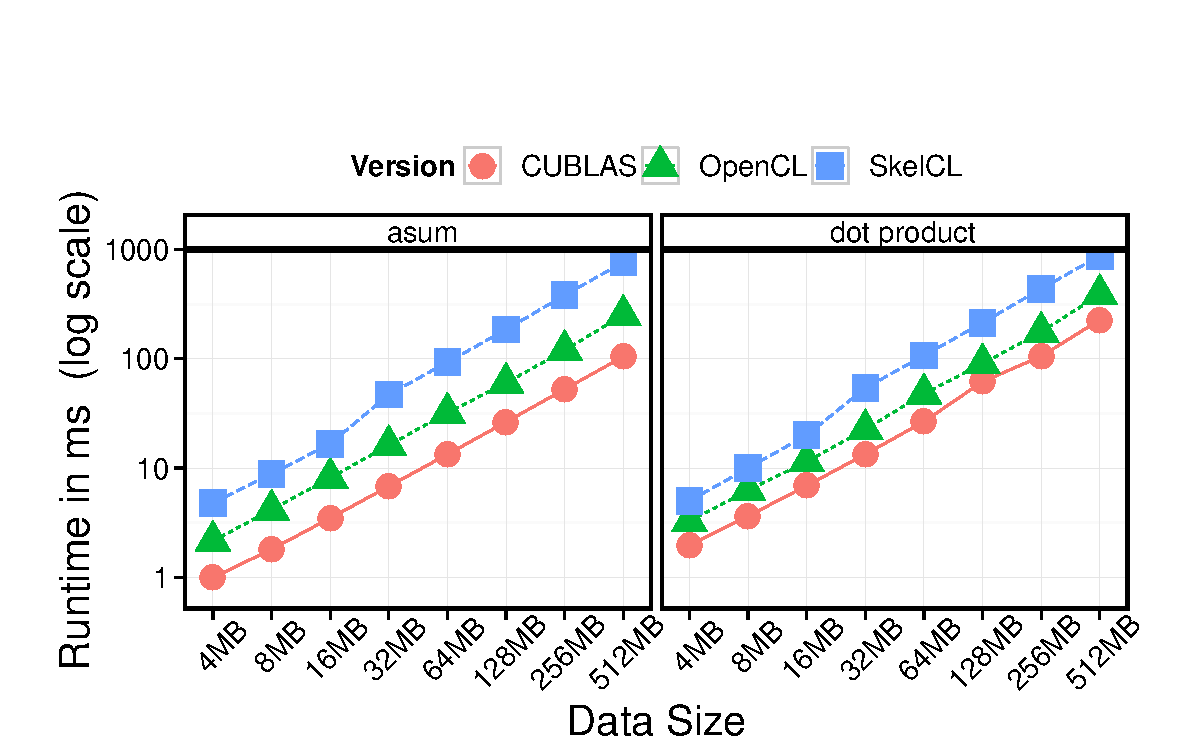
\includegraphics[width=1.2\textwidth]{Plots/Asum/asum.pdf}
    \caption{Runtime for \emph{asum}.}
    \label{fig:skelcl:asum}
  \end{subfigure}
  \hfill
  \begin{subfigure}[t]{.45\textwidth}
    \hspace{-.1\textwidth}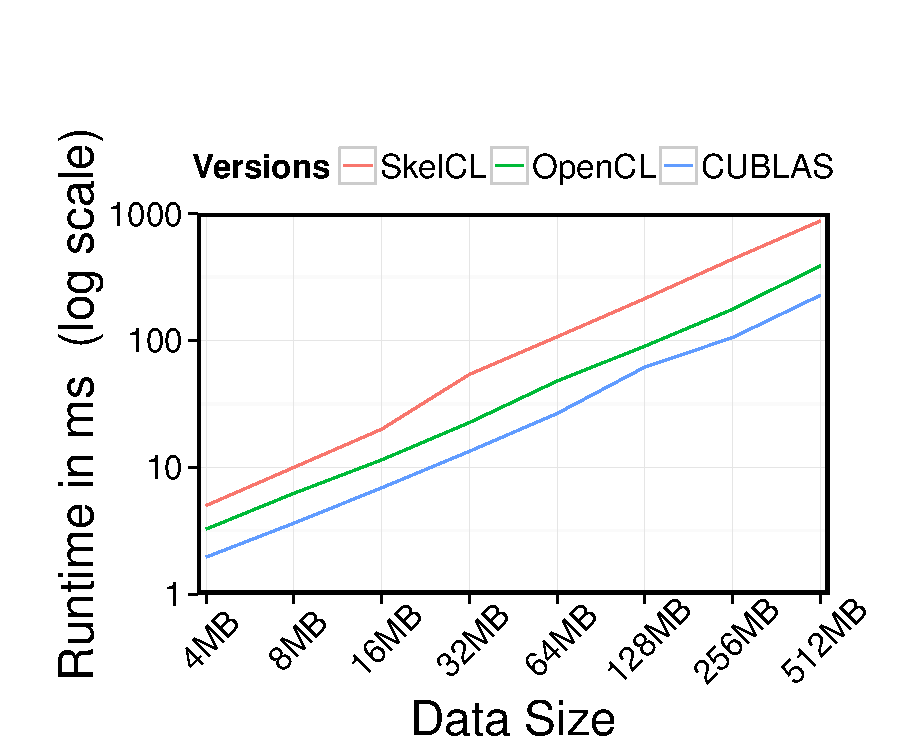
\includegraphics[width=1.2\textwidth]{Plots/DotProduct/dotProduct.pdf}
    \caption{Runtime dot product.}
    \label{fig:skelcl:dot}
  \end{subfigure}
\end{figure}

\subsection*{Discussion}

\begin{figure}[tb]
  \centering
  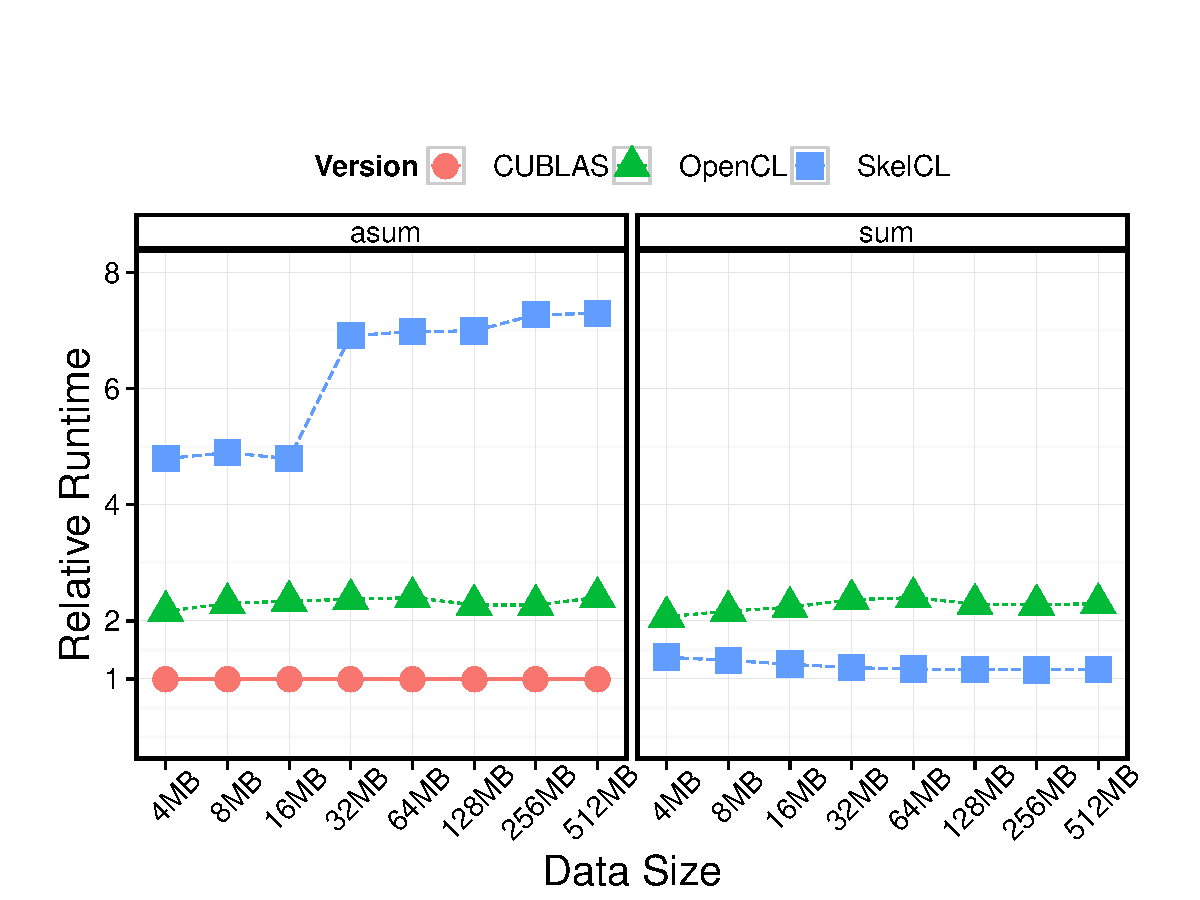
\includegraphics[width=.9\textwidth]{Plots/Reduce/reduce.pdf}
  \caption{Relative runtime compared to CUBLAS of the naive \OpenCL and \SkelCL versions of \emph{asum} and reduce.}
  \label{fig:skelcl:reduce}
\end{figure}
As discussed in \autoref{chapter:skelcl} the \SkelCL library implementation generates one \OpenCL kernel for each skeleton (and two for the \reduce skeleton).
This procedure makes it difficult to \emph{fuse} multiple skeleton implementations into a single \OpenCL kernel, which would be required to achieve a competitive performance for the \emph{asum} and dot product benchmark.

To validate this explanation and quantify the effect of launching additional kernels we measured the performance of \SkelCL's \reduce skeleton on its own.
This measurement is similar to the \emph{asum} benchmark, but without applying the \map skeleton for obtaining the absolute value of every element, \ie, we measured the \emph{sum} benchmark:
\begin{equation}
  sum\ \vec{x} = reduce\ (+)\ 0\ \vec{x}
  \label{eq:sum}
\end{equation}
For comparison we also changed the naive \OpenCL implementation of \emph{asum} to not apply the absolute value function to every element.
\autoref{fig:skelcl:reduce} shows the performance results of the naive \OpenCL version and the \SkelCL version for \emph{asum} on the left and \emph{sum} on the right.
The plots show the performance relative to the performance of the CUBLAS implementation of \emph{asum}.
We can see, that the performance difference for \emph{asum} and \emph{sum} it is very small (only up to $4$\%) for the naive \OpenCL version.
This makes sense, as the most part of the computation is spend for reducing the elements and not for applying a simple function to each element.
For the \SkelCL implementations the difference between the two benchmarks is very large.
This is due to the fact that for \emph{asum} a separate \OpenCL kernel is launched which reads each value from the global memory, applies the absolute value function to it, and stores the result back to global memory.
The reduction kernel then starts by reading each element back from global memory.
This leads to a huge difference in runtime, where the \emph{asum} benchmark is up to $6.2$ times slower than the \emph{sum} benchmark.
Furthermore, we can see that for the \emph{sum} benchmark the \SkelCL implementation outperforms the naive \OpenCL implementation and is only between $16$\% and $37$\% slower than the CUBLAS \emph{asum} implementation.

In \autoref{ch:fifth}, we will discuss a novel compilation technique which addresses this challenge.
This technique supports the generation of a single efficient OpenCL kernel for applications like the \emph{asum} and dot product examples.

